\chapter{第三期}

\section{2019年10月8日星期三 阴}

许亦凡

今天,我在写作业时。突然妈妈说了一句话:“我带了一个好吃的东西。”我嘴里流着口水说:“是什么好吃的东西呀!”我妈妈继续说:“是许亦凡牌手指!”我们家的人都哄堂大笑起来,原来我太饿了,把手指放到嘴巴里“尝”了!

\section{2019年10月9日 星期三 阴}

陈姿伊

今天我们家的小狗“上吊”啦,“汪!汪汪!汪汪汪!”在我写作业的时候,笼子里传来了响亮的狗叫,还伴随着“咣当咣当”的声音,我把注意力从作业本上移到了狗笼上,那一刻,我惊呆了,只见那只小狗雪球两只爪子搭在侧门上,那张虽然小却长满尖牙的嘴紧紧地咬住上面那扇门,两只脚都腾空了,但还是有一只小脚时不时的蹬一下笼子底部,细小的狗胡子也轻轻地摆动着。这样子活像上吊呀!

“雪球!”我大喝一声,“快给我下来!”雪球听见了,吓了一大跳,嘴松开了,四只小脚也“嗒”的一声落了地,他肯定是以为自己可以把门打开,跳出来玩呢!

\section{2019年10月10日 星期四 晴}

陈思涵

我的弟弟个子不高,头倒是挺大。你可别小瞧他这大大的头,这个大头啊,不仅有那些水分,还“塞”了不少知识呢!弟弟虽然只有三岁,但他可聪明了!一次,我们一家去初中操场运动。只见弟弟飞快地跑向杠杆,先把手放在一个杆上,脚踏地,脚用力一蹬,放在了另一个杆上。弟弟爬杆像猴子一样,眨眼间,他已经爬了一半,但他不敢下来了,我只好上前把他抱了下来。你说,这位大头弟弟是不是聪明又搞笑呢?

\section{2019年10月10日 星期四 晴}

杨若君

今天晚上我在写作业的时候有个题想不出来。我一边想一边吸着笔,不知道怎么回事,突然觉得嘴里有股很苦的怪味。我一看笔,啊!我竟然把笔里的墨汁给吸出来了。我慌极了,趁爸爸不注意,赶紧去卫生间漱口,一看镜子满嘴都是黑的。都漱了两大杯了,吐出来的唾沫还是黑的,我漱了老半天才漱干净,可我的舌头还是有点黑,以后我再也不敢吸笔了。

\section{2019年10月10日 星期四 多云}

张欣瑜

漫步在两旁皆是树木的小路上,满眼都是落叶。我随手捡起一片树叶,仔细地观察着。原来是枫叶。瞧,她多美呀!那向周围伸展的叶片,多像我张开五指的手掌啊,边缘略呈锯齿状。上面的叶脉清晰可见,很有条理地串联在一起。它的颜色更是美轮美奂,就好比那正要熊熊燃烧的烈火,那么鲜艳夺目。我知道,枫叶不仅有耀眼的红色,还有黄色、绿色等一系列迷人的颜色。我爱秋天的枫叶!

\section{2019年10月10日 星期四 晴}

徐诚磊

今天,我放学被留了下来。我写作文写得很慢,又跟赵祺钰聊天,所以快放学也没写完。我心乱如麻,一心想着放学,于是赶紧乱写一通就交上去了。结果老师说:“这是什么东西,重写!”老师的话如同在我头上泼了一盆凉水。我知道按时放学是不可能了,又要被妈妈骂一通了。我垂头丧气地回到座位上重写了,等大部队走了好久,才重写完成。以最快的速度收拾好书包回家去了,果不其然,我真的被妈妈骂了一通。

\section{2019年10月11日 星期二 晴}

孙轩睿

下课时,我正在上厕所,不经意之间瞄了眼窗外,马上就惊呆了:瞧,有一棵树上长满了“黄金”,而且还长了几个“翡翠”!我很想去捡一点儿便宜,于是决定上好厕所确定一下,如果是就赶紧支捡。
上好厕所,我来到窗边,仔细一看,原来只是一棵皂角树,现在已经秋天了,树的叶当然要黄了!于是就被我看成了黄金,而“翡翠”则是还没有变黄的绿叶。
哎,就知道不可能“树上长黄金.”真是白高兴一场。

\section{2019年10月14日 星期一 阴转小雨}

陈思涵

在上个星期六,学校为我们四年级举办了一次“十岁成长礼”。其中,最让我感动的是与家长互读信。我拿出信封,认认真真地读了起来。读完后,爸爸妈妈一起拿出信,也专心致志地读了起来。听着听着,我的眼圈渐渐红了起来,我被爸爸妈妈写的信感动了。过了一会儿,两行眼泪流过鼻头,滚过脸颊,落在了草地上。我想,爸爸妈妈对我们的爱,用笔是写不尽的,更是一样无价之宝。十年来,他们经历风吹雨打,却丝毫不畏惧,永远做我们的后盾。我想对你们说一声“谢谢你们!”

\section{2019年10月14日,星期一 阴}

赵奕麟

在今天清晨当我睡得朦朦胧胧的时候,我听到妈妈的菜刀在砧板上打着节拍,小鸟“叽叽喳喳”唱着愉快的歌,还听到了碗在水池里“乒乒乓乓”的发出声响,风儿“呼呼”的吹来,清晨的小区可真是一个乐团啊!

\section{2019年10月14日 星期一 雨}

张欣瑜

学校里的桂花开了。远看,桂花树像一把撑开的绿色的大伞,我远远地就闻到了一股清香,那清香令我贪婪的吸了几口,我东张西望想找桂花,只见那一团团的桂花球,像一个个小棉花球。满树的桂花闪着金黄色的光芒,特别耀眼。近看,桂花树的叶子翠绿,两头尖尖,特别茂盛。我通过绿叶,在绿叶丛中发现了桂花,我仔细观赏,只见它小巧玲珑的,有四片花瓣,还有几丝花蕊。一阵微风拂过,桂花飘落下来,就像金黄色的蝴蝶翩翩起舞。校园里的桂花真是太漂亮了!

\section{2019年10月15日 星期二 晴}

孙轩睿

今天晚上,我的水笔没墨了,笔芯在椅子旁的柜子里。我去拿,发现在最里面,就把头探了进去,很快就拿到了,我把头向上伸,想赶紧换好笔芯,却忘了头在柜子里。“咚”我的头撞到了顶,撞得眼冒金星,满眼的星星,并不自觉地转了起来,又“咚”的一声,原来头转到顶时又撞到了顶。我感觉星星多了好多,然后我又使劲让头停下来。过了几秒头停下来了。
“呜”我以后不把头伸进柜子里了,我要用两根铁棍夹。

\section{2019年10月16日 星期三 晴}

蒋鲁弋

昨天晚上。我正在睡觉,突然听见一阵哭的声音,我走近妈妈的房间,发现弟弟在里面哭,他又滚又跳,又喊又叫,声音大极了!我当作没事,又回去睡觉,但声音太响了,吵得我睡也睡不着觉,我滚来滚去,过了好久,那个声音终于消失了,我长叹一口气,看了一下闹钟,不看不知道,一看吓一跳,已经12点了,我马上睡觉,过了一会儿,进入了梦乡。第二天早上,太阳照在我的身上,我觉得舒服极了,又换了个角度晒太阳,这时候老妈过来了,他把我的被子拉掉,对我大声说:“起床啦!”我慢慢的坐了起来,一看已经8点了,我马上去穿衣服,一边穿一边说:“可恶的闹闹,害我迟到,我恨你!”

\section{2019年10月16日 周三 晴}

宋闵俊

今天,我觉得眼睛很酸,就揉了一下它,哎呦喂,双眼睛反而更酸了!这时,眼保健操的音乐响了起来,我闭上了眼睛,心想:“真是天助我也!可以好好休息了!”果然,做完眼保健操,眼睛就不酸了。

\section{2019年10月16日 星期三 晴}

余蕙琳

家里的客厅就是一个小小的植物园。餐桌上的金桂如同一颗颗黄金,再佩上它碧绿碧绿的叶子,真是无语伦比的美。再看看上面亭亭玉立的玫瑰,它的红似血一样,仿费它是花中的女王一样。把眼睛往右看,能看到两盆茂盛的绿萝,绿萝嫩得特别好看,犹其是它垂落在花盆外的茎。在书画作品下,点缀着一瓶情人草,白紫花瓣星星点点地布满枝干,在情人草的旁边,你会看到一种可爱的植物,那便是多肉,多肉真是多肉,它的叶子真的是十分饱满。在电视机旁,还有一株枝叶舒展的富贵竹,越上面,富贵竹的叶子越嫩。家里最显眼的是窗户边的红掌,从底面看,红色的叶子像一片片爱心,上面则是像一个个小小的玉米一样的花蕊,看起来真是独一无二!你喜不喜欢我家的小小植物园呢?

\section{2019年10月16日 星期三 晴}

蒋欣恬

今天晚上我在看书,一只蚊子边叫边飞进我的“领土”,在我的手背上咬了一口又大又红的包,我想,叫你天天给我塞红包,我今天非要打你个头破血流!于是我放下书站起来打蚊子。我跳起来,爬下去,左打右打,
可还是打不着蚊子。我气愤的走开了,扔下一句话:“蚊子,我打算在家里放上蚊香给你,君子报仇,十年不晚,走着瞧。”

\section{2019年10月17日 星期四 晴}

徐诚磊

今天快放学了,来欣年突然说:“第三组的`高效组'评比已经满十次了”。我暗暗惊道:“不会吧,他们都可以换蛋糕了!”放学了,只见詹老师拿着一大堆蛋糕走了过来,给第三组每人一块。詹老师还让他们都站在后面,给他们拍了一张合照。拍完照,他们就开始吃了。“哇,是巧克力夹心蛋糕!”我馋得“口水直流三千尺”。我想起了我们组:陈浩然写得很慢,而他前面的我们几个都是泥菩萨过河——自身难保,所以我们组才拿了两次“高效组”。接下来我们组要加把劲了,争取早日拿到十次“高效组”。

\section{2019年10月18日 星期五 晴}

沈冠屹

晚上,老妈不在。我可以痛痛快快看许多书了!我一本接一本地看去。当老妈回来时已经八点多了。可那时,我却一个作业也没有写,老妈看见了,骂得我落花流水,还让我马上写完。写着写着,老妈看了一下钟说:“现在太晚了,不许写了,明天早上再写,去睡觉!”妈呀,我真是惨不忍睹啊!看来我以后不能再这么晚写作业了呀!

\section{2019年10月21日 星期一 晴}

来欣年

今天,我到学校的时候,发现有一个同学走在我的前面---姜妍慧。我的心里想出了一个念头:我可以偷偷走在她的身后,趁她不注意吓她一下。想完,我蹑手蹑脚的跟在她后面,深怕她看到我了,等我们一前一后走了一会到了楼梯拐角,我想这是个好机会,就推了她一把,她转过身被我吓得愣住了。

\section{2019年10月22日 星期二 晴}

戴瑞彤

最近几天,妹妹班里停课了,因为他们班里有两个人得了手足口病,老师怕会传染,才让他们班停课的。妈妈正带着妹妹出去玩,我趁着这个功夫,在家里偷偷玩起了手表。我的心里忐忑不安,七上八下的。突然,我的脚下发出“叭”的一声,我一下子把手表扔在床上,打开作业本,假装开始写作业。这时,我定睛一看,原来是我的橡皮掉在了地上。忽然,有一个人拍了一下我的头,说:“在找什么东西呢?地上有钱吗?”我一看,原来是妈妈回来了,我连忙拿起笔,写起了作业,心想下次还是不要玩手表好。

\section{2019年10月22日 星期二 晴}

许亦凡

清早,我被厨房冲牛奶的声音吵醒,揉揉惺忪的睡眼,望了望床前的闹钟,哇!七点半啦!我跳下床,三步并作两步地跨到书桌前,赶着收拾我的书包。心里默默地想:不要迟到呀!

\section{2019年10月22日 星期二 晴}

蒋鲁弋

今天放学的时候,爸爸拿来一堆东西,放在桌子上,高兴地对我说:“儿子,你看!”我往那堆东西望去,吃惊地看着。那堆里面有个“领头雁”的大奖杯,有一张红红的荣誉证书,还有一条长长的锦旗…… 这时,爸爸语重心长地跟我说:“儿子,你要知道,这些东西是爸爸努力才得来的,所以你干什么事情都要用尽全力,才能收获满满。”听了老爸的话,我下决心要努力学习,当一个优秀的小学生。

\section{2019年10月22日 星期二 晴}

孙轩睿

我正哼着歌,走在回家路上,突然“轰”的一声巨响,把我吓了一大跳。我的脑海里瞬间涌入了好多电影里的场景:恐怖分子把炸弹放在高楼里,炸断了高楼;突然开始打仗,有人扔了一颗手雷,手雷炸了;或者是有飞机来轰炸我们滨江。想到这里,我赶紧四下看了看,发现周围的楼房好好的,没断也没有烟;马路上也没有枪声;天上蓝天白云,轰炸机的影子也没有。“卖爆米花喽,香喷喷的爆米花……”一个声音响起。只见一个大爷坐在地上,左边放着个“大炮”爆米花机,面前摆着几罐爆米花,香气扑鼻。

\section{2019年10月23日 星期三 晴}

今天放学回家,我看到了感人的一幕,一位清洁工正在扫垃圾,他的头发蓬乱,细小无神的眼睛,塌塌的鼻子,不成比例地镶在一张黑黑的脸上。突然,一个男生骑着自行车飞驰而过,正好骑在了臭水洼上,溅了一旁的清洁工一身的污水。那位清洁工回过头来,用细小的眼睛望着已经离他而去的男生,茫茫然的脸上显露出一副难以名状的神色--是愤怒?但很快他又笑了笑,似乎原谅了那位男生,理解了他的无意。我继续向前走,一边走一边想,清洁工在有些人眼中十分低贱,其实,清洁工这个工作与老师、建筑工一样高尚,他们默默无闻、无私奉献,不到生命最后一刻,就不会停止他们的工作,有时他们受到了误解,却毫无任何怨言,流眼泪也是躲在角落自己偷偷地红眼圈。这件事让我懂得了如何做人:做人就要无私奉献于社会,不顾一切。

\section{2019年10月23日 星期一 晴}

许智涵

今天回到家,我一眼就发现了一个灰白白、胖嘟嘟的大家伙,他就是我们的新朋友——大冰箱!这冰箱比旧的宽一倍,矮点,打开一看,真大!我一边想着这个冰箱被外婆带来的菜塞满的样子,一边笑着做作业去了。

\section{2019年10月24日 星期四 晴}

孙轩睿

昨天编程课刚上课,老师就问了我们一个问题:“你们会九九乘法表吗?如果会的话今天我们就做一个。”一听要做东西,大家不高兴了,于是故意一起说:“不会!我们不会那个九什么什么法什么。”老师知道我们在演戏,于是说:“我不信,你们背给我听!”我们想了想,互相交换了一下眼神,大家都同意演戏演到底,既然大家都同意,那么就开始吧,我们面向老师,一本正经地坐好,开始说了起来:“一一得八十,三三得八……”,反正我们没做九九乘法表。

哎,与其说是一班编程高手,不如说是一班戏精啊!

\section{2019年10月24日 星期四 晴}

徐诚磊

今天吃过晚饭,我看见妈妈很累,就主动提议:“我来洗碗吧!”妈妈点了点头。这时我记起,上次看到的生活小妙招——用水果套来洗碗。说干就干,我拿来一个水果套,挤上一点洗洁精,开始洗碗了。我搓呀搓,不一会儿就出现了许多泡泡。我一只碗一只碗地搓过去,泡泡越来越丰富。换作以前用抹布洗碗,泡泡越搓越少。用水果套来洗碗真是既干净又环保,我建议大家可以回家去试试哦!

\section{2019年10月24日 星期四 晴}

蒋鲁弋

今天早晨,我怀着兴奋的心情来到学校,拿出铁环,放在桌子上,然后大声说:“谁没有铁环,来我这儿拿!”同学们呼啦一下围了上来,你一言我一语地说道:“给我一个”“我还没有”“我要三个”…… 我一个个地分给大家。这时,老师来了,她看到我不在早读,而是在发铁环,生气地说道:“早读不认真读,把这袋东西交上去!”我惭愧地把铁环交了上去,委屈地坐回座位上。但这件事是我的错,我不该在早读的时间起哄,影响大家早读,希望老师能原谅我,还请您把铁环分给大家。

\section{后记}

过去的几个月,在詹老师,各位同学和各位家长的努力下,《闲言碎语》活动继续坚持着。詹老师每天要花大量的时间批阅每位同学们的笔记,感谢老师的默默付出。同学们更是辛苦,在完成作业和各种培训班的空余时间还要绞尽脑汁写一篇日记,确实不容易。家长们也积极响应,百忙之中抽时间把孩子的文章打印成电子稿发过来。总之,在大家的共同努力下,有了我们这一期的闲言碎语。

闲言碎语的初衷是鼓励大家能坚持写作,提高写作水平。我上学时经常语文不及格,写作水平不好,常为此而遗憾。写作是一项非常有价值的技能,前几天听吕丽娟老师的讲座说:“执笔人有历史解释权”。意思是说,后人眼中的事实,是由前人笔下的文章所描绘的。所以,能写好文章是一件神圣的事情。如果读到一篇与自己想法一致的文章,作者写出了你想要说的话,那是多么地畅快。希望大家能体会到写作的重要性,不仅仅是为了应付考试,更是为了能更好的表达自己。

在公众号发布的每日之最,只是为了鼓励同学们的积极性,同时希望通过这样一个仪式,鞭策大家能一起坚持下去。没有选中的同学切莫灰心,家长也切勿打消他们的积极性。

另外,想跟大家分享写作方法。我不是专家,所以不敢胡言乱语,且引用林语堂先生关于写作的建议。第一,写作如作画,可分为临帖和写生。临帖就是要多看书,模仿前辈的方法进行写作。本期中一位同学描写自然景物的文字,观察细致入微,文字生动优美。定是她平时积累的写作素材比较多。写生就是自己创作了。第二,初级阶段可以以描写文和叙事文为主。他认为因为阅历比较少,刚开始比较难以写出议论文。描写文和叙事文写好了以后,写议论文,也就功到自然成了。本期中大多数同学写的就是叙事文,其中有位同学讲述了家中的一件小事,她在写的时候把自己感动得眼泪吧嗒吧嗒直落,旁人读了,也深为感动。请相信,能感动自己的事,也一定能感动他人。所以,写出心中所想,记下感动自己的事,也一定能感动读者。

最后,祝大家暑期愉快,四年级再见。


\begin{figure}[htb]
    \centering
    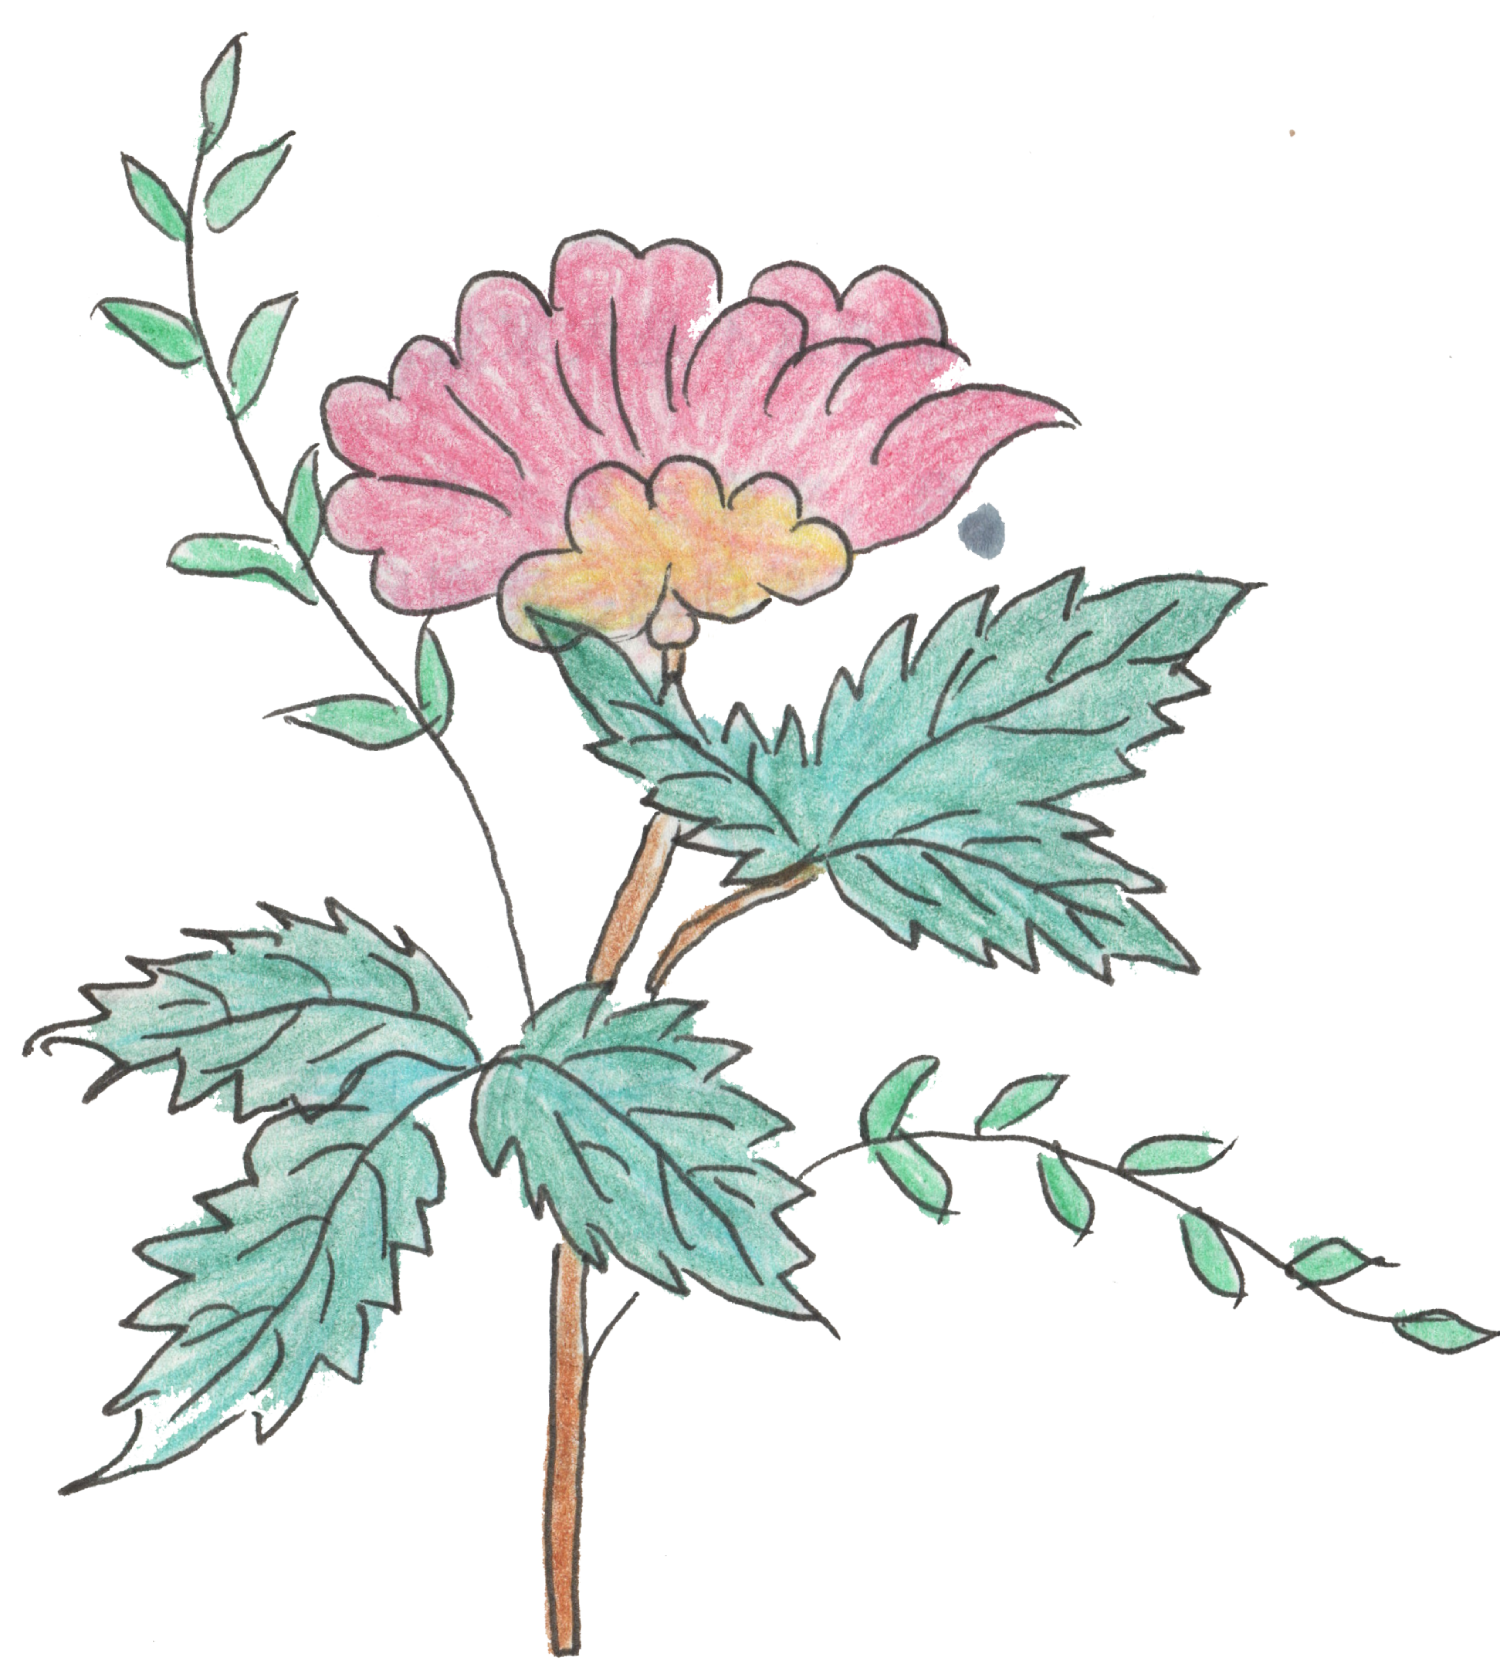
\includegraphics[width=0.8\textwidth]{figure/03.png}
\end{figure}